\documentclass[12pt, a4paper]{article}
\usepackage{polyglossia}
\usepackage{geometry}
\usepackage{lua-ul}
\usepackage{color,soul}
\usepackage[dvipsnames, HTML]{xcolor}
\usepackage{pifont}
\usepackage{hyperref}
\usepackage{graphicx}
\usepackage[protrusion]{microtype}
\usepackage[absolute]{textpos}
\usepackage{adjustbox}

\setlength\parindent{0pt}


\setmainfont{AlegreyaSans}
\newfontfamily\fonthead{AlegreyaSansSC}
\newfontfamily\fontsub{Alegreya}

%sections
\newcommand{\head}[1]{
  \phantomsection
  \section*{\centering{\fonthead{#1}}}
  \addcontentsline{toc}{section}{#1}
}

\newcommand{\subhead}[1]{
  \phantomsection
  \subsection*{\centering{\fontsub{#1}}}\vspace{1em}
  \addcontentsline{toc}{subsection}{#1}
}


\newcommand{\subheadfoot}[2]{
  \phantomsection
  \subsection*{\texorpdfstring{\centering\fontsub{#1\protect\footnote{#2}}}{#1}}\vspace{1em}
  \addcontentsline{toc}{subsection}{#1}
}


\newcommand{\subsubhead}[1]{
  \phantomsection
  \subsubsection*{\fontsub{#1}}
  \addcontentsline{toc}{subsubsection}{#1}
}


\newcommand{\quotehead}[2]{
  \phantomsection
  \subsubsection*{\texorpdfstring{\fontsub{\textit{#1}}}}
  \addcontentsline{toc}{subsubsection}{#2}
}


\newcommand{\titlehead}[2]{
\begin{center}
{\fonthead
\textbf{\huge{#1}}\\[0.1in]
\LARGE{#2}\\[0.3in]
}
\end{center}
}

\newcommand{\ind}{\hspace{1.5em}}

\newcommand\note[1]{
  \begin{textblock*}{6cm}(17cm,1cm)
  \fonthead
  \rotatebox{-25}{\textbf{#1}}
\end{textblock*}
}


\begin{document}

\newgeometry{top=0.5in,bottom=0.7in}

\titlehead{Emma}{Jane Austen}


\subhead{Overview \& Plot}

\ind Emma, a \underLine{comedy of manners} set in \underLine{Highbury} about Emma's 
struggle with blindness and her fear of confronting her own feelings which leads
her to meddle harmfully in the lives of others. The novel uses free indirect discourse
where the narrator\footnote{\, an anonymous who tells the reader how characters feel and think,
and who also provides insight and commentary.}
steps in and out of Emma’s thoughts. It is narrated in the third person and 
the immediate past tense. It sometimes uses flashbacks,\footnote{\, is when the linear
sequence of narration is cut and it goes back to the past events.} to provide information about
earlier events, and foreshadowing,\footnote{\, a narrative device where a writer hints at 
events that will occur later in the story.} to provide hints about the future. The below 
diagram shows the structre of the plot:



\begin{figure}[ht]
  \centering
  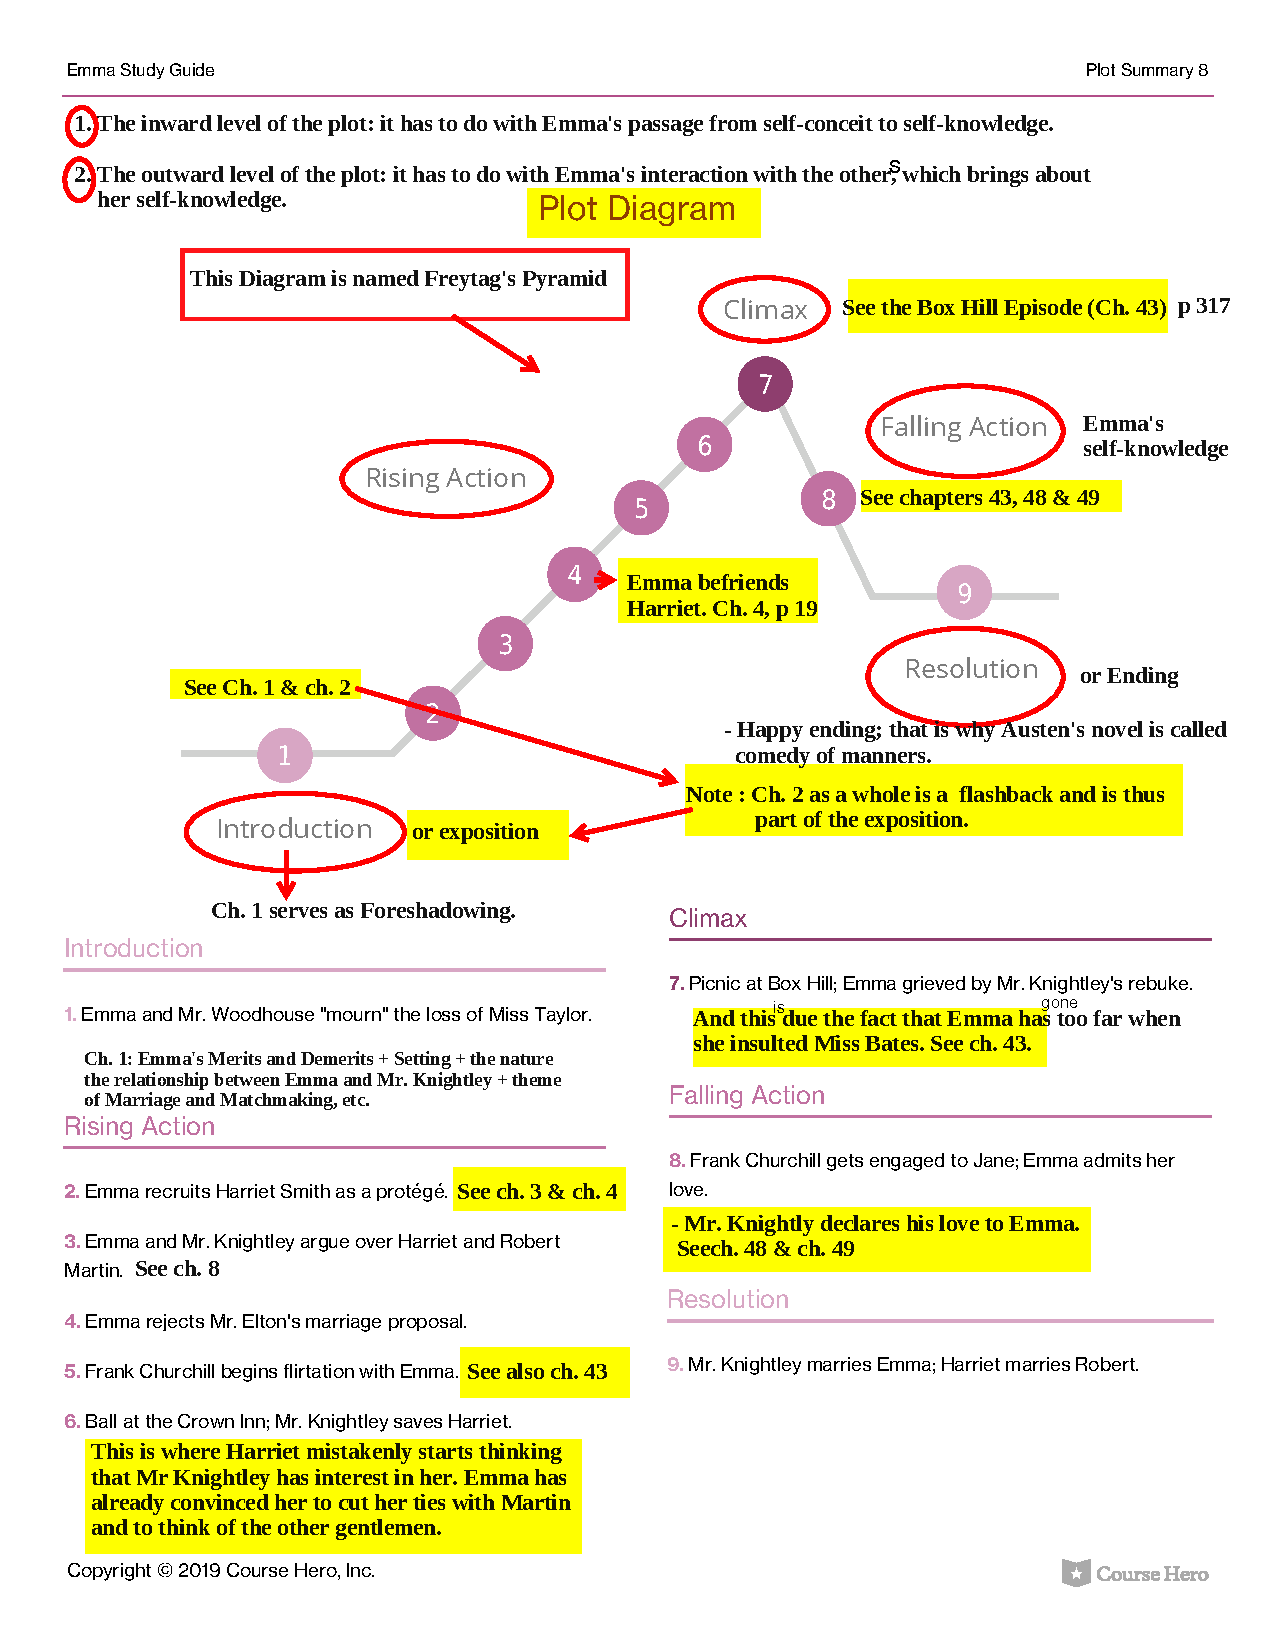
\includegraphics[width=0.9\textwidth]{diagram.pdf}
\end{figure}

\newpage
\subhead{Characters \& Estate}


\begin{itemize}

  \item \textbf{Hartfield}, where Mr. Woodhouse (Henry) and Emma live.
  \item \textbf{Randalls}, where the Westons live.
  \item \textbf{Enscombe}, where the Churchills  live.
  \item \textbf{Donwell Abbey} where Mr. Knightley live.
  \item \textbf{Abbey-Mill Farm} where the Martins live, it is part of Downwell Abbey.
  
\end{itemize}


\begin{figure}[ht]
  \centering
  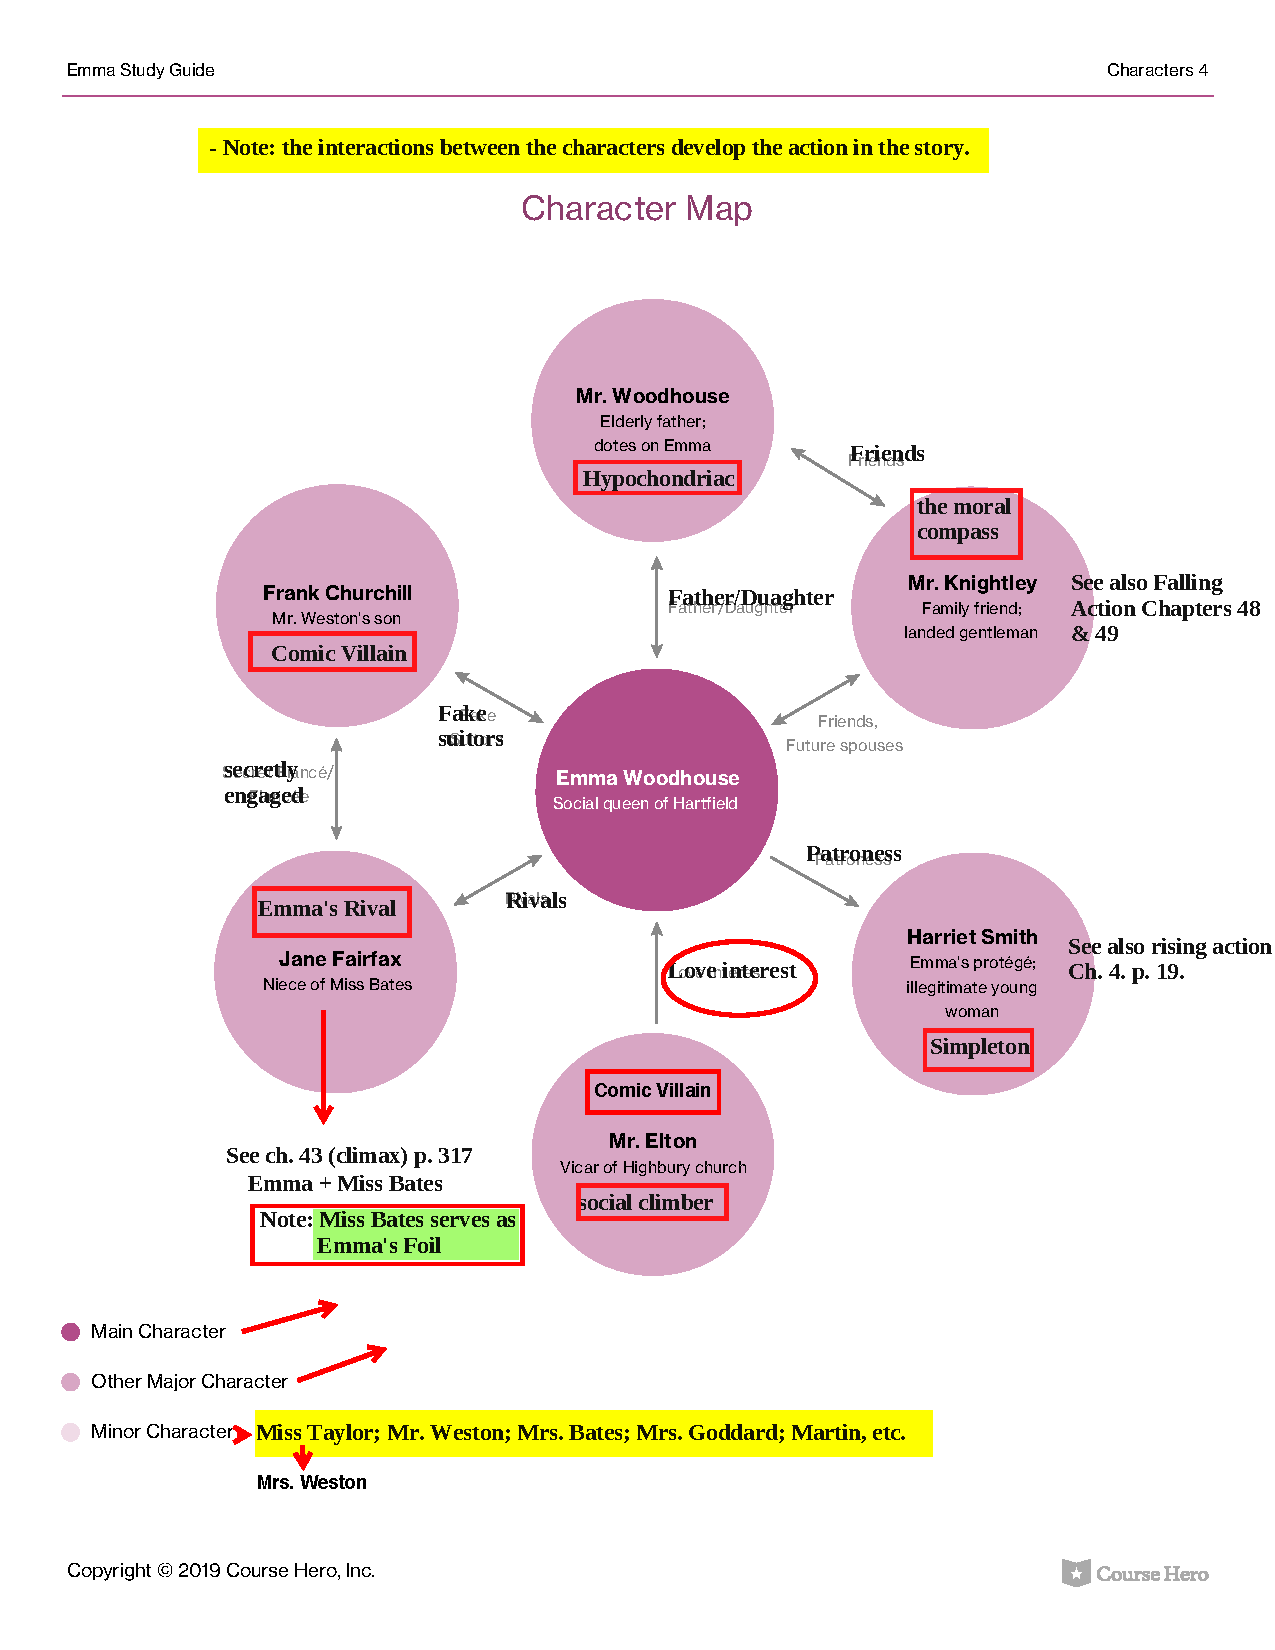
\includegraphics[width=0.9\textwidth]{characters.pdf}
\end{figure}

\restoregeometry


\subhead{Draw a Character Sketch of the Following}

\subsubhead{Emma Woodhouse}

Handsome, clever, rich, and somewhat spoiled. She is twenty one when the story opens.
Her mother died when she was five, after that Miss Taylor became her governess.
She has been mistress of the house since her older sister got married. Although smart, 
she lacks the discipline to practise or study anything in depth. She is
portrayed as compassionate to the poor, but at the same time has a
strong sense of class status (snobbish). Being spoiled and vain makes her blind to 
her feelings and the feelings of others, and she ends up hurting both.

\subsubhead{Mr. Knightley}

George Knightley is a gentleman and a longtime family friend of the Woodhouse family.
He is considerate, aware of the feelings of the other characters, and 
always exhibits good behaviour and judgment.
He is the moral compass of the story and Emma's only critic. He owns Donwell Abbey where the Martins
have a farm. He is thirty-seven when the story opens and the elder brother 
of Mr. John Knightley, the husband of Emma's elder sister Isabella.

\subsubhead{Harriet Smith}

Beautiful, naive, and fair, with a fine bloom, blue eyes, light hair,
regular feature, and a look of great sweetness. She was seventeen when the story opens.
She is the illegitimate daughter of somebody. She lived with Mrs. Goddard. Emma
becomes her friend and takes her under her wing. However, she turns out to be a bad influence
on Harriet because she projects her own desires and beliefs onto her. 

\subsubhead{Mr. Elton}

Good-looking, well-mannered, and ambitious. Twenty seven years old and unmarried when the story opens.
He gets his living by being the vicar of Highbury and he lives alone in the vicarage. He
is a social climber, he wants to marry a wealthy woman so he go up the social ladder. After Emma
rejects him, he soon marries Miss Hawkins, proving he never truly cared for Emma.

\newpage
\subsubhead{Mr. Henry Woodhouse}

Is the father of Emma and the owner of Hartfiled. He is generous and well mannered,
although his hypochondriac\footnote{\,
a person who is abnormally anxious about their health.} nature and his hate for change
make it a somewhat difficult for others to get along with him. He enjoys keeping a small circle of 
people around him and only invites them to his own house on his own terms. He is the reason Emma does not consider marriage, 
because marriage is the origin of change. Despite being self-centered and unable to see beyond his own feelings,
he is kind and well-respected by others.

\subsubhead{Miss Bates}

Is an old, alright looking, poor spinster who lived with her mother 
and spent most of her youth caring for her. She was simple 
and cheerful which made her popular in Highbury. She loved everybody and was 
interested in everybody's happiness. She was full of trivial communications
and harmless gossip. She is considered to be Emma's foil because she lack all the
merits Emma has.

\subsubhead{Mr. Weston}

Is a kind and cheerful man who enjoys people’s company, and was a native of Highbury.
After joining the militia he marries Miss Churchill and they have a son named Frank,
soon after Miss Churchill dies and due to financial struggles Mr. Weston, decided
to give Frank to the Churchills family to take care of him. Later, after establishing 
himself in trade and marrying Miss Taylor, he moved with her to live at Randalls.

\subsubhead{Frank Churchill}

Is handsome, charming, and witty. He is Mr Weston's son by his first marriage but 
was raised by his wealthy aunt and uncle, the Churchills, at the family estate of Enscombe 
in Yorkshire. He is revealed over the course
of the novel to be a scheming, insincere, and somewhat cowardly man. 
He manipulates and plays games with the other characters to ensure his secret engagement 
to Jane remains concealed.

\subsubhead{Jane Fairfax}

Is an orphan whose only family is her aunt, Miss Bates, and her grandmother, Mrs Bates.
Though a native of Highbury, she was educated and nurtured by the
Campbells, who had been friends of her father. She is a beautiful, bright, and elegant woman
but because of her unpleasant situation, she is destined to be a governess. She is secretly 
engaged to Frank Churchill. She is considered as Emma’s rival though she is far more accomplished,
which makes Emma envy her.



\subhead{Identify, explain and comment on the following quotations}



\quotehead{Quote 1/ 
"Emma Woodhouse, handsome,
clever, and rich, with comfortable
home and happy disposition,
seemed to unite the best
blessings of existence; and had
lived nearly twenty one years in
the world with very little to
distress or vex her." 
}{Quote 1}

These words are said by the narrator in the exposition about the hero of the novel, Emma.
She is described as having the best that life can offer. However, the narrator uses an ironic tone
which makes us wonder; is Emma going to make use of her merits? 


\quotehead{Quote 2/
"The real evils, indeed, of Emma’s situation were the power of having rather too much her
own way, and a disposition to think a little too well of herself: these were the disadvantages
which threatened alloy to her many enjoyments. The danger, however, was at present so
unperceived, that they did not by any means rank as misfortunes with her."
}{Quote 1}

These words are said by the narrator in the exposition about Emma's demerits. The narrator foreshadows the novel’s
structure as a whole: Emma having too much of her way and her vanity makes her blind to her
feelings and the feelings of others. This causes her to meddle in the life of others, harming both them and herself.

\quotehead{Quote 3/
"A young farmer ... is the very last
sort of person to raise my
curiosity. The yeomanry are
precisely the order of people with
whom I feel I can have nothing to
do."
}{Quote 2}

These words are said by Emma about Robert Martin when she was talking with Harriet.
She reveals a shocking degree of snobbery in her desire to distance herself from Martin.
As a result, she tries to make Harriet lose interest in Martin.


\quotehead{Quote 4/
"I confess that I have seldom seen
a face or figure more pleasing to
me that hers. But I am a partial old
friend."
}{Quote 3}

These words are said by Mr. Knightley about Emma when he was talking to Mrs. Weston.
She pushes him to acknowledge Emma's physical beauty, but he hardly wants to
admit his attraction, undercutting his statement by saying he may be partial because he is an old friend.

\quotehead{Quote 5/
"Till it appears that men are much
more philosophic on the subject of
beauty than they are generally
supposed; till they do fall in love
with well-informed minds instead
of handsome faces, a girl, with
such loveliness as Harriet, has a
certainty of being admired and
sought after, of having the power
of choosing from among many."
}{Quote 5}

These words are said by Emma when she was arguing with Mr. Knightley about
whether Martin is a good fit for Harriet. She responds that Harriet's
beauty give her the privilege to choose, and that men only care about
beauty when looking for a wife.

\quotehead{Quote 6/
"The first error, and the worst, lay at her door. It was foolish, it was wrong, to take so active a
part in bringing any two people together. It was adventuring too far, assuming too much,
making light of what ought to be serious—a trick of what ought to be simple. She was quite
concerned and ashamed, and resolved to do such things no more."
}{Quote 1}

These words are said by the narrator about Emma's reflections after Mr. Elton proposes to her.
She realize how wrong she was in thinking him attached to Harriet. 
She understands what is wrong with matchmaking: that courtship should
be serious and simple; it should flow naturally between two people.

\quotehead{Quote 7/
"You are very fond of bending little
minds; but where little minds
belong to rich people in authority, I
think they have a knack of swelling
out, till they are quite as
unmanageable as great ones."
}{Quote 7}

These words are said by Emma to Mr. Knightley when they were talking about Frank Churchill.
After Knightley criticizes Frank for not fulfilling his duty as a son, Emma defends him saying
that he lives under the influence of his aunt who keeps him away from Highbury. In this dialogue she shows her great
use of wit and metaphor.

\quotehead{Quote 8/
"And no great harm if it does, said
Mr. Woodhouse. 'The sooner every
party breaks up, the better."
}{Quote 6}

These words are said by Mr. Woodhouse to Mr. Weston when the latter was trying to persuade him
to allow Emma to stay out late when she attends the Coles' dinner party. Mr. Woodhouse comment
show his self-centeredness and selfishness.

\quotehead{Quote 9/
"Why really, dear Emma, I say that
he is so very much occupied by
the idea of not being in love with
her, that I should not wonder if it
were to end in his being so at last."
}{Quote 9}

\quotehead{Quote 10/
"She did ... regret the inferiority of
her own playing and singing. She
did most heartily grieve over the
idleness of her childhood—and sat
down and practiced vigorously an
hour and a half."
}{Quote 10}

\quotehead{Quote 11/
"She was vexed beyond what could have been expressed—almost beyond what she could
conceal. Never had she felt so agitated, so mortified, grieved, at any circumstance in her life.
She was most forcibly struck. The truth of his representation there was no denying. She felt it
at her heart. How could she have been so brutal, so cruel to Miss Bates! How could she have
exposed herself to such ill opinion in any one she valued! And how suffer him to leave her
without saying one word of gratitude, of concurrence, of common kindness!"
}{Quote 1}


\quotehead{Quote 12/
"She is poor; she has sunk from
the comforts she was born to; and,
if she live to old age, must
probably sink more. Her situation
should secure your compassion. It
was badly done, indeed!"
}{Quote 9}

\quotehead{Quote 13/
"Emma’s eyes were instantly withdrawn; and she sat silently meditating, in a fixed attitude,
for a few minutes. A few minutes were sufficient for making her acquainted with her own
heart. A mind like hers, once opening to suspicion, made rapid progress; she touched, she
admitted, she acknowledged the whole truth. Why was it so much worse that Harriet should
be in love with Mr. Knightley than with Frank Churchill? Why was the evil so dreadfully
increased by Harriet’s having some hope of a return? It darted through her with the speed of
an arrow that Mr. Knightley must marry no one but herself!"
}{Quote 1}

\quotehead{Quote 14/
"Seldom, very seldom, does
complete truth belong to any
human disclosure; seldom can it
happen that something is not a
little disguised, or a little mistaken;
but where, as in this case, though
the conduct be mistaken, the
feelings are not, it may not be very
material."
}{Quote 10}


\subhead{Provide short answer for each of the following questions}

\subsubhead{What Emma's merits ?}

\subsubhead{What are Emma's demerits ?}

\subsubhead{Who was suffering from intellectual solitude and why ?}

\subsubhead{Who was described as suffering from blank solitude and Why ?}

\subsubhead{Why is Miss Bates considered Emma’s foil ? }

\subsubhead{Who are The Martins and why Emma wanted Harriet to cut her relationship with them ?}

\subsubhead{Why Emma thinks Elton as a suitable future husband to Harriet ?}


\subhead{Fill in the Blank}

\begin{itemize}

\item The new vicar that comes to Highbury after the death of Mrs. Bates' husband is \underLine{Mr. Elton}.

\item \underLine{Mr. George Knightley} considered as the moral compass in Emma's life.

\item Emma take place in a village called \underLine{Highbury}.
  
\end{itemize}



\subheadfoot{Emma Major Motifs}{\, a motif is a recurring symbol, idea, or image that appears across a story to develop
its major themes.}


\subsubhead{Bad Parenting}

\ind In Emma we see few characters being bad parents to their children:
The first is Mr. Woodhouse (Henry), his fastidious nature and hatred of change prevent 
Emma from even considering marriage. The second is Weston, after facing financial struggles, 
he abandons his son Frank, leaving him in the care of his late wife’s relatives (the Churchills)
The third is Harriet's parents, they abandon her in childhood leaving her in the custody of
Mrs. Goddard’s.


\subsubhead{Blindness}

\ind In Emma, few characters show blindness to the truth because of their biases and desires.
We see it in Emma when she misunderstands the motives of Mr. Elton, thinking  
that he is in love with Harriet while he actually has feelings for Emma. Her desire
to match Mr. Elton with Harriet blinds her to his true feelings. Similarly,
when she speaks cruelly of Jane Fairfax, it stems from her jealousy of Jane’s accomplishments. We also see
this blindness in Mr. Knightley; he criticizes Frank Churchill not on the basis of truth, but rather 
out of jealousy because of Frank's relationship with Emma.

\subsubhead{Visits}

\ind The main events of the novel take place during visits that the characters pay to each other. The
frequency and length of visits between characters indicates the level of intimacy and attachment
between them. Frank’s frequent visits to Hartfield show his relationship with Emma to be close.
Mr. Knightley’s constant presence at Hartfield indicates his affection and regard for Emma.
Emma encourages Harriet to limit a visit with the Martin family to fifteen minutes, because such a
short visit clearly indicates that any former interest has been lost. 

\subsubhead{Parties}

\ind In Emma, parties center on social conventions more than around
individual attachments. Emma’s hosting a dinner party for Mrs. Elton, a woman she dislikes,
exemplifies this characteristic. There are six important parties in the novel: the Christmas Eve party at
Randalls, the dinner party at the Coles’, the dinner party given for Mrs. Elton, the dance at the Crown
Inn, the morning party at Donwell Abbey, and the picnic at Box Hill. Each occasion provides characters 
with opportunities to observe one another and witness social interactions.



\end{document}
